% Prezentacja Beamer -- Wieloskalowa agentowa symulacja pandemii
% Dawid Mularczyk, WI AGH, 2026

\documentclass[polish,10pt]{beamer}

\usepackage[utf8]{inputenc}
\usepackage[T1]{fontenc}
\usepackage[polish]{babel}
\usepackage{booktabs}
\usepackage{tabularx}
\usepackage{graphicx}
\usepackage{amsmath}
\usepackage{xcolor}
\usepackage{caption}

\usetheme{Madrid}
\usecolortheme{whale}
\setbeamertemplate{navigation symbols}{}
\setbeamertemplate{caption}[numbered]

\newcolumntype{Y}{>{\small\centering\arraybackslash}X}

% ---- STOPKA: lewa kolumna = Dawid Mularczyk - WI AGH ----
\author[Dawid Mularczyk -- WI AGH]{Dawid Mularczyk}
\institute[WI AGH]{Wydział Informatyki, Akademia Górniczo-Hutnicza\\[4pt]
  \texttt{muldaw@student.agh.edu.pl}}
\title[Symulacja pandemii -- ABM]{Wieloskalowa agentowa symulacja\\
  rozprzestrzeniania się pandemii wirusowej}
\subtitle{Projekt studencki -- Etapy 1, 2 i~3}
\date{2026}

% ============================================================
\begin{document}

\begin{frame}
  \titlepage
\end{frame}

\begin{frame}{Plan prezentacji}
  \tableofcontents
\end{frame}

% ============================================================
\section{Motywacja i model SEIRD}

\begin{frame}{Motywacja -- dlaczego modelowanie agentowe?}
  \begin{columns}[T]
    \column{0.48\textwidth}
    \textbf{Klasyczne modele ODE (SIR)}
    \begin{itemize}
      \item Jednorodne mieszanie populacji
      \item Brak struktury przestrzennej
      \item Brak heterogeniczności jednostek
    \end{itemize}
    \[
      \frac{dS}{dt} = -\beta \frac{SI}{N},\;\;
      \frac{dI}{dt} = \beta \frac{SI}{N} - \gamma I
    \]

    \column{0.48\textwidth}
    \textbf{Modelowanie agentowe (ABM)}
    \begin{itemize}
      \item Każdy agent: własne atrybuty i reguły
      \item Realistyczna topologia miejska (graf POI)
      \item Emergentne zjawiska (superspreaderzy, ogniska)
      \item Naturalne testowanie interwencji
    \end{itemize}
  \end{columns}

  \vspace{0.5cm}
  \begin{block}{Cel projektu}
    Trójstopniowa implementacja wieloskalowej symulacji ABM pandemii
    w~środowisku miejskim opartym na~węzłach POI z~modelem SEIRD.
  \end{block}
\end{frame}

\begin{frame}{Model epidemiologiczny SEIRD}
  \[
    S \xrightarrow{\lambda(t)} E \xrightarrow{\sigma} I \xrightarrow{\gamma} R,
    \qquad I \xrightarrow{\mu} D
  \]

  \begin{columns}[T]
    \column{0.55\textwidth}
    \begin{itemize}
      \item \textbf{S} -- Podatny (brak odporności)
      \item \textbf{E} -- Inkubacja (zainfekowany, niezakaźny, mobilny)
      \item \textbf{I} -- Zakaźny (emituje patogen)
      \item \textbf{R} -- Wyleczony (nabyta odporność)
      \item \textbf{D} -- Zgon
    \end{itemize}
    \vspace{0.3cm}
    \textbf{Ładunek wirusowy} -- ciągła zmienna agenta:\\
    narasta pod koniec fazy E, szczytuje w~I,\\
    maleje przy zdrowieniu. Bezpośrednio skaluje siłę zakażenia.

    \column{0.42\textwidth}
    \begin{tabular}{ll}
      \toprule
      Parametr & Wartość \\
      \midrule
      Inkubacja & 4 dni \\
      Zakaźność & 8 dni \\
      $p_{\text{death}}$ & 2\% \\
      $p_{\text{mult}}$ & 0,16 \\
      Cel $R_0$ & 2,5--3,5 \\
      \bottomrule
    \end{tabular}
  \end{columns}
\end{frame}

% ============================================================
\section{Architektura systemu}

\begin{frame}{Środowisko: Graf węzłów POI}
  \begin{columns}[T]
    \column{0.50\textwidth}
    Graf $G=(V,E)$ -- węzły to fizyczne lokalizacje:

    \begin{itemize}
      \item \textbf{Gospod.\ domowe:} $\lfloor N/4 \rfloor$ węzłów, ~4 os./dom
      \item \textbf{Biura:} $\lfloor N/25 \rfloor$, ~25 pracowników
      \item \textbf{Szkoły:} $\lfloor N/30 \rfloor$, ~30 uczniów
      \item \textbf{Sklepy:} $\lfloor N/50 \rfloor$
      \item \textbf{Parki:} $\lfloor N/100 \rfloor$
      \item \textbf{Placówki zdrowia:} $\lfloor N/200 \rfloor$
    \end{itemize}
    \vspace{0.2cm}
    \small Skalowanie proporcjonalne do $N$ zapobiega efektowi
    \textit{super-węzła} (setki agentów w 3 biurach).

    \column{0.48\textwidth}
    \begin{tabular}{lc}
      \toprule
      Typ węzła & $p_{\text{base}}$ \\
      \midrule
      Gospod.\ domowe & 0,35 \\
      Szkoła & 0,30 \\
      Biuro & 0,20 \\
      Placówka zdrowia & 0,15 \\
      Sklep & 0,10 \\
      Park & 0,03 \\
      \bottomrule
    \end{tabular}

    \vspace{0.35cm}
    \textbf{Dzienny harmonogram:}\\
    Dom $\to$ Praca/Szkoła $\to$ Sklep? $\to$ Park?\\
    {\small (zablokowane przy lockdownie / SD)}
  \end{columns}
\end{frame}

\begin{frame}{Mechanizmy transmisji i atrybuty agentów}
  \begin{columns}[T]
    \column{0.52\textwidth}
    \textbf{Transmisja wewnątrz węzła:}
    \[
      P_{\text{inf}} = \Bigl(1 - \prod_{i}(1-p_{\text{eff},i})^{v_i}\Bigr)
        \cdot (1 - \text{immunity})
    \]
    Modifikatory $p_{\text{eff}}$: maseczki $(\eta_M=0{,}5)$,\\
    dystans społeczny $(-20\%)$,\\
    higiena $h = 1 - 0{,}6\cdot(\bar{\Theta}_H - 0{,}5)$.

    \begin{alertblock}{\texttt{MAX\_INFECTIOUS\_CONTACTS = 5}}
      Każdy podatny losuje co najwyżej 5 zakaźnych\\
      agentów -- eliminuje saturację w dużych węzłach.
    \end{alertblock}

    \column{0.46\textwidth}
    \textbf{Kluczowe atrybuty agenta:}

    \begin{tabular}{ll}
      \toprule
      Atrybut & Rola \\
      \midrule
      \texttt{age} & mobilność, śmiertelność \\
      \texttt{viral\_load} & siła emisji \\
      \texttt{immunity} & podatność \\
      \texttt{wears\_mask} & $\times(1-\eta_M)$ \\
      \texttt{hygiene\_score} & czynnik $h$ \\
      \texttt{contact\_rate} & pr.\ wizyt \\
      \texttt{vaccinated} & $-80\%$ zgonów \\
      \bottomrule
    \end{tabular}

    \vspace{0.2cm}
    \begin{block}{Superspreader}
      CR~$=3{,}0$;\; $\Theta_H=0{,}1$
    \end{block}
  \end{columns}
\end{frame}

% ============================================================
\section{Etap 1 -- Prototyp MVP}

\begin{frame}{Etap 1: Prototyp MVP na siatce}
  \begin{columns}[T]
    \column{0.46\textwidth}
    \textbf{Środowisko:} siatka $50\times50$, topologia torusowa

    \textbf{Populacja:} $N=500$, 5\% startowo zakaźnych

    \textbf{Ruch:} losowy (sąsiedztwo Moore'a), $p_{\text{inf}}=0{,}20$

    \vspace{0.3cm}
    \textbf{Wyznaczenie emergentnego $R_0$:}
    \[
      \bar{k} = 8 \cdot 0{,}20 \cdot 0{,}95 \approx 1{,}52
    \]
    \[
      R_0 \approx 0{,}20 \cdot 1{,}52 \cdot 8 \approx \mathbf{2{,}4}
    \]

    \begin{block}{Weryfikacja}
      Stochastyczne $R_0 \approx 2{,}6$\\
      Zgodne z~[2,0;\;3,5] dla\\
      wirusów oddechowych.
    \end{block}

    \column{0.52\textwidth}
    
\includegraphics[width=\textwidth]{epidemic_curve.png}

    \vspace{0.1cm}
    {\small\textit{Krzywe SEIRD, MVP ($N=500$, 100 kroków). Szczyt I ok.\ dnia~25.}}
  \end{columns}
\end{frame}

% ============================================================
\section{Etap 2 -- Implementacja POI}

\begin{frame}{Etap 2: Implementacja i naprawione błędy}
  \begin{columns}[T]
    \column{0.52\textwidth}
    \textbf{3 krytyczne błędy naprawione w~Etapie~2:}

    \begin{enumerate}
      \item \textbf{Super-węzeł} -- skalowanie liczby węzłów z~$N$;
            np.\ $N=500$: 125 domów, 20 biur, 16 szkół.
      \item \textbf{Mega-autobus} -- tranzyt grupowany po \emph{konkretnym}
            węźle~ID (nie po typie POI); pierwotnie wszyscy jadący do ,,biur''
            wchodzili do jednego pojazdu $\Rightarrow R_0 \gg 10$.
      \item \textbf{Saturacja} -- \texttt{MAX\_INFECTIOUS\_CONTACTS = 5}
            eliminuje nierealistyczną kumulację siły zakażenia.
    \end{enumerate}

    \vspace{0.2cm}
    \textbf{Kalibracja końcowa:}\\
    $p_{\text{mult}} = 0{,}16$ $\Rightarrow$ $R_0 \approx 2{,}5$,
    attack rate $\approx 75\%$

    \column{0.46\textwidth}
    \textbf{Stos technologiczny:}
    \begin{itemize}
      \item \textbf{Python 3} + \textbf{Mesa} (ABM)
      \item \textbf{NetworkX} -- graf POI
      \item \textbf{Streamlit} -- dashboard
      \item \textbf{HTML5 canvas} -- real-time
      \item \textbf{pytest} -- 25 testów
    \end{itemize}

    \vspace{0.3cm}
    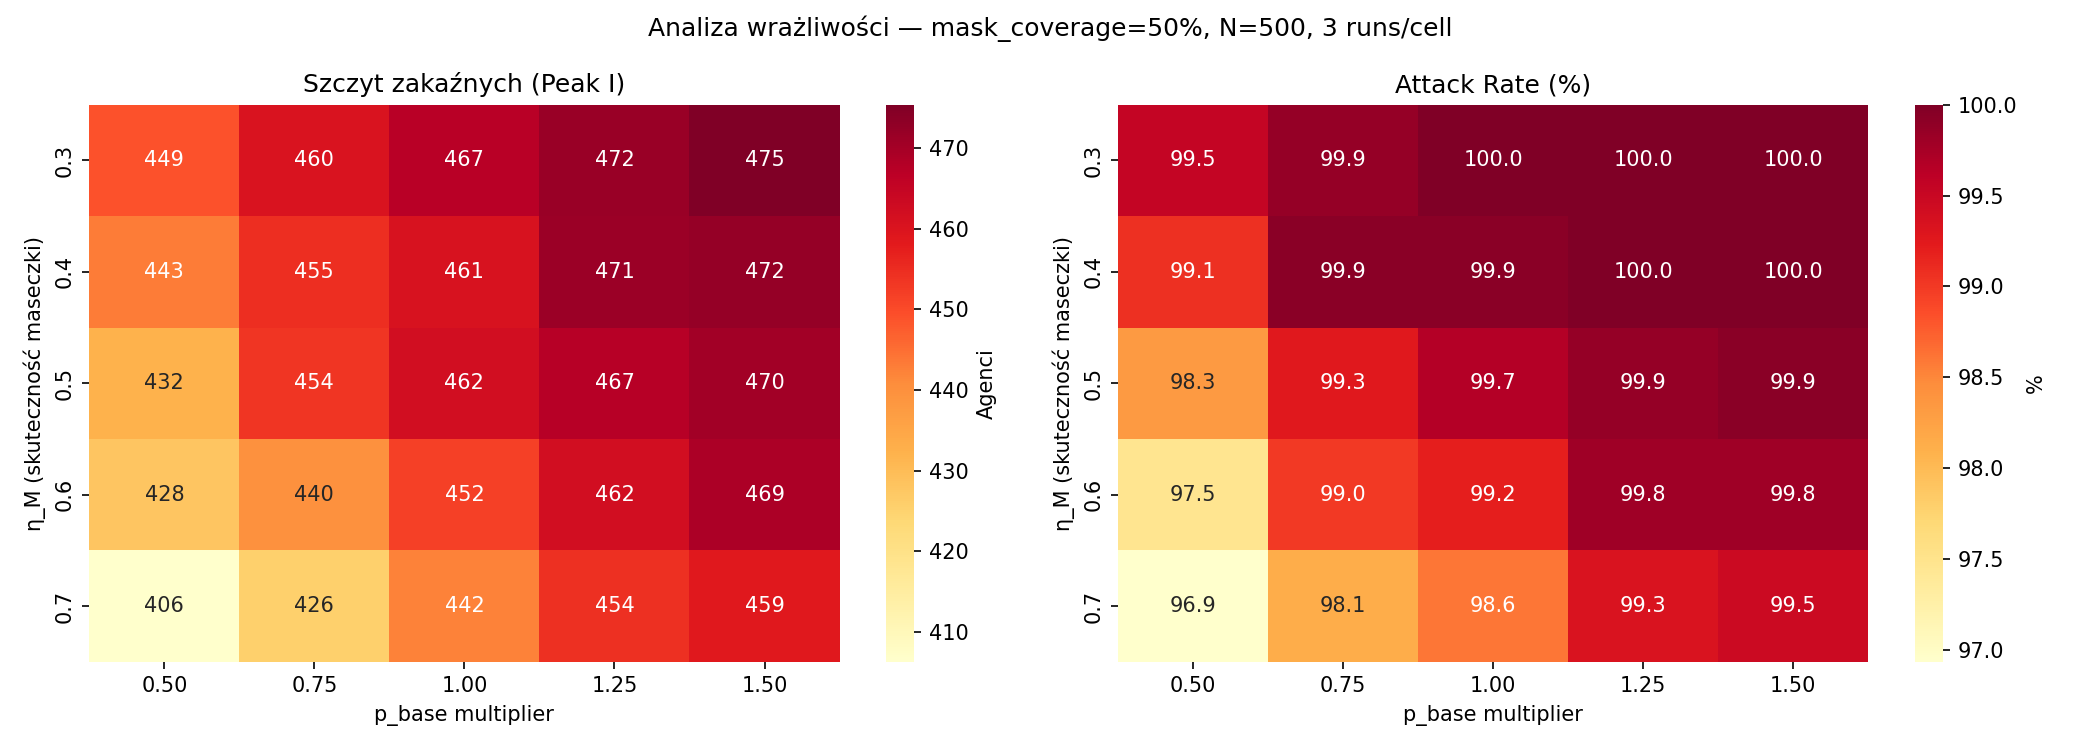
\includegraphics[width=\textwidth]{sensitivity_heatmap.png}

    \vspace{0.1cm}
    {\small\textit{Analiza wrażliwości: peak~I i~AR\\
    vs.\ $p_{\text{mult}}$ i $\eta_M$.}}
  \end{columns}
\end{frame}

\begin{frame}{Etap 2: Interfejs aplikacji}
  \begin{columns}[T]
    \column{0.50\textwidth}
    \textbf{Dashboard Streamlit}\\
    {\small Parametry, wykresy SEIRD i~statystyki końcowe}

    \vspace{0.15cm}
    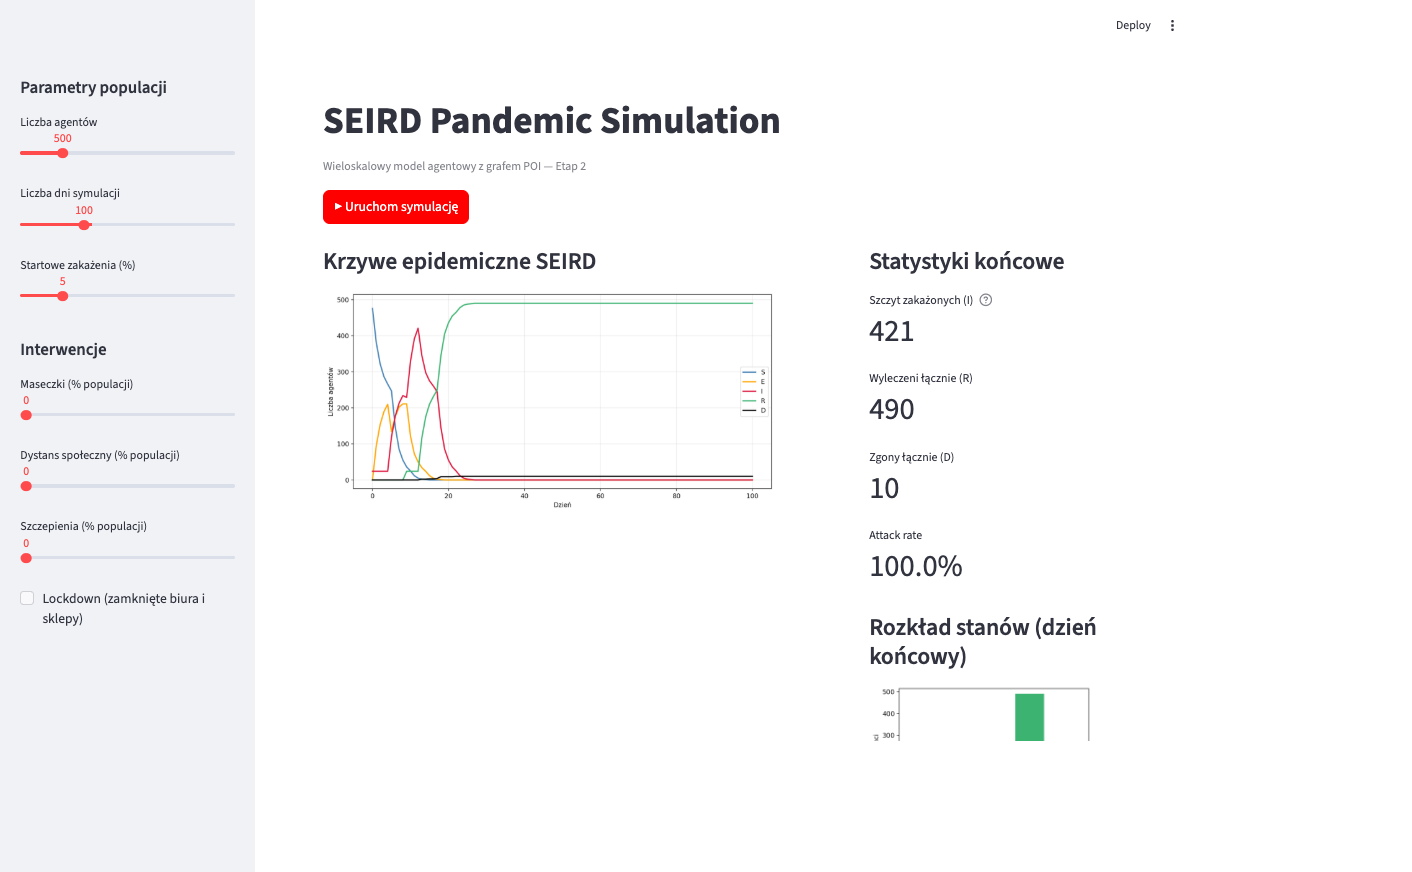
\includegraphics[width=\textwidth]{screenshot_dashboard.png}

    \column{0.48\textwidth}
    \textbf{Animacja real-time (canvas)}\\
    {\small Agenci poruszają się między węzłami POI.\\
    Interwencje aplikowane \emph{na~żywo}, bez restartu.}

    \vspace{0.15cm}
    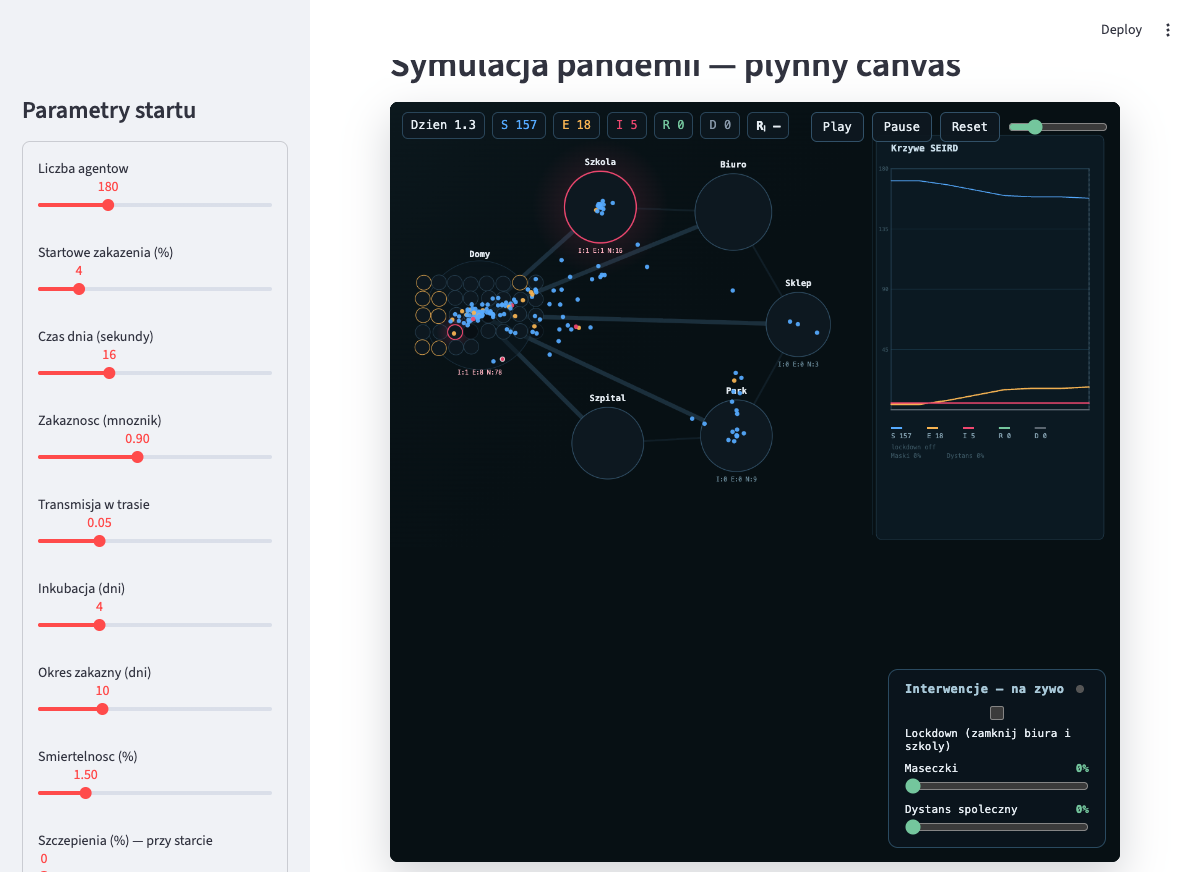
\includegraphics[width=\textwidth]{screenshot_canvas.png}
  \end{columns}

  \vspace{0.3cm}
  \begin{block}{Kluczowa zaleta real-time canvas}
    Włączenie lockdownu lub maseczek w~trakcie epidemii i~natychmiastowa
    obserwacja spłaszczenia krzywej -- bez restartowania symulacji.
  \end{block}
\end{frame}

% ============================================================
\section{Etap 3 -- Eksperymenty}

\begin{frame}{Etap 3: Metodologia -- 5 scenariuszy}
  \begin{block}{Konfiguracja bazowa}
    $N=500$ \textbullet{} 7~powtórzeń (różne ziarna) \textbullet{} 180~kroków\\
    Inkubacja 4~dni, zakaźność 8~dni, $p_{\text{death}}=2\%$,
    $p_{\text{mult}}=0{,}16$, start: 2\% zakaźnych
  \end{block}

  \vspace{0.3cm}
  \begin{tabularx}{\textwidth}{@{}lX@{}}
    \toprule
    \textbf{Scenariusz} & \textbf{Zmiana vs.\ bazowy} \\
    \midrule
    1. Bazowy & Brak interwencji -- punkt odniesienia \\
    2. Lockdown & Zamknięcie biur, szkół, sklepów \\
    3. Szczepienia 60\% & \texttt{immunity}=0,5; redukcja zgonów o~80\% \\
    4. Superspreaderzy 5\% & CR=3,0;\; $\Theta_H=0{,}1$ dla 25 agentów \\
    5. Wysoka higiena & $\bar{\Theta}_H=0{,}85$ (bazowo~0,50) \\
    \bottomrule
  \end{tabularx}

  \vspace{0.3cm}
  Wykresy: \textbf{mediana} 7~powtórzeń + pasmo IQR (percentyle 25.--75.)
\end{frame}

\begin{frame}{Wyniki: Baseline i Lockdown}
  \begin{columns}[T]
    \column{0.46\textwidth}
    \textbf{Sc.~1 -- Baseline:}
    \begin{itemize}
      \item Attack rate: \textbf{75,1\%}
      \item Peak~I: \textbf{88} agentów (dzień~31)
      \item Zgony: \textbf{7};\quad $R_0 \approx 2{,}5$
    \end{itemize}

    \vspace{0.4cm}
    \textbf{Sc.~2 -- Lockdown:}
    \begin{itemize}
      \item Attack rate: \textbf{3,5\%}\quad\textcolor{teal}{$\downarrow$96\%}
      \item Peak~I: \textbf{14} (dzień~8)
      \item Zgony: $<1$
    \end{itemize}

    \begin{block}{Dlaczego tak skuteczny?}
      Przecięcie wszystkich pozadomowych ścieżek transmisji.
      Pozostaje tylko klaster domowy o~ograniczonym zasięgu.
    \end{block}

    \column{0.52\textwidth}
    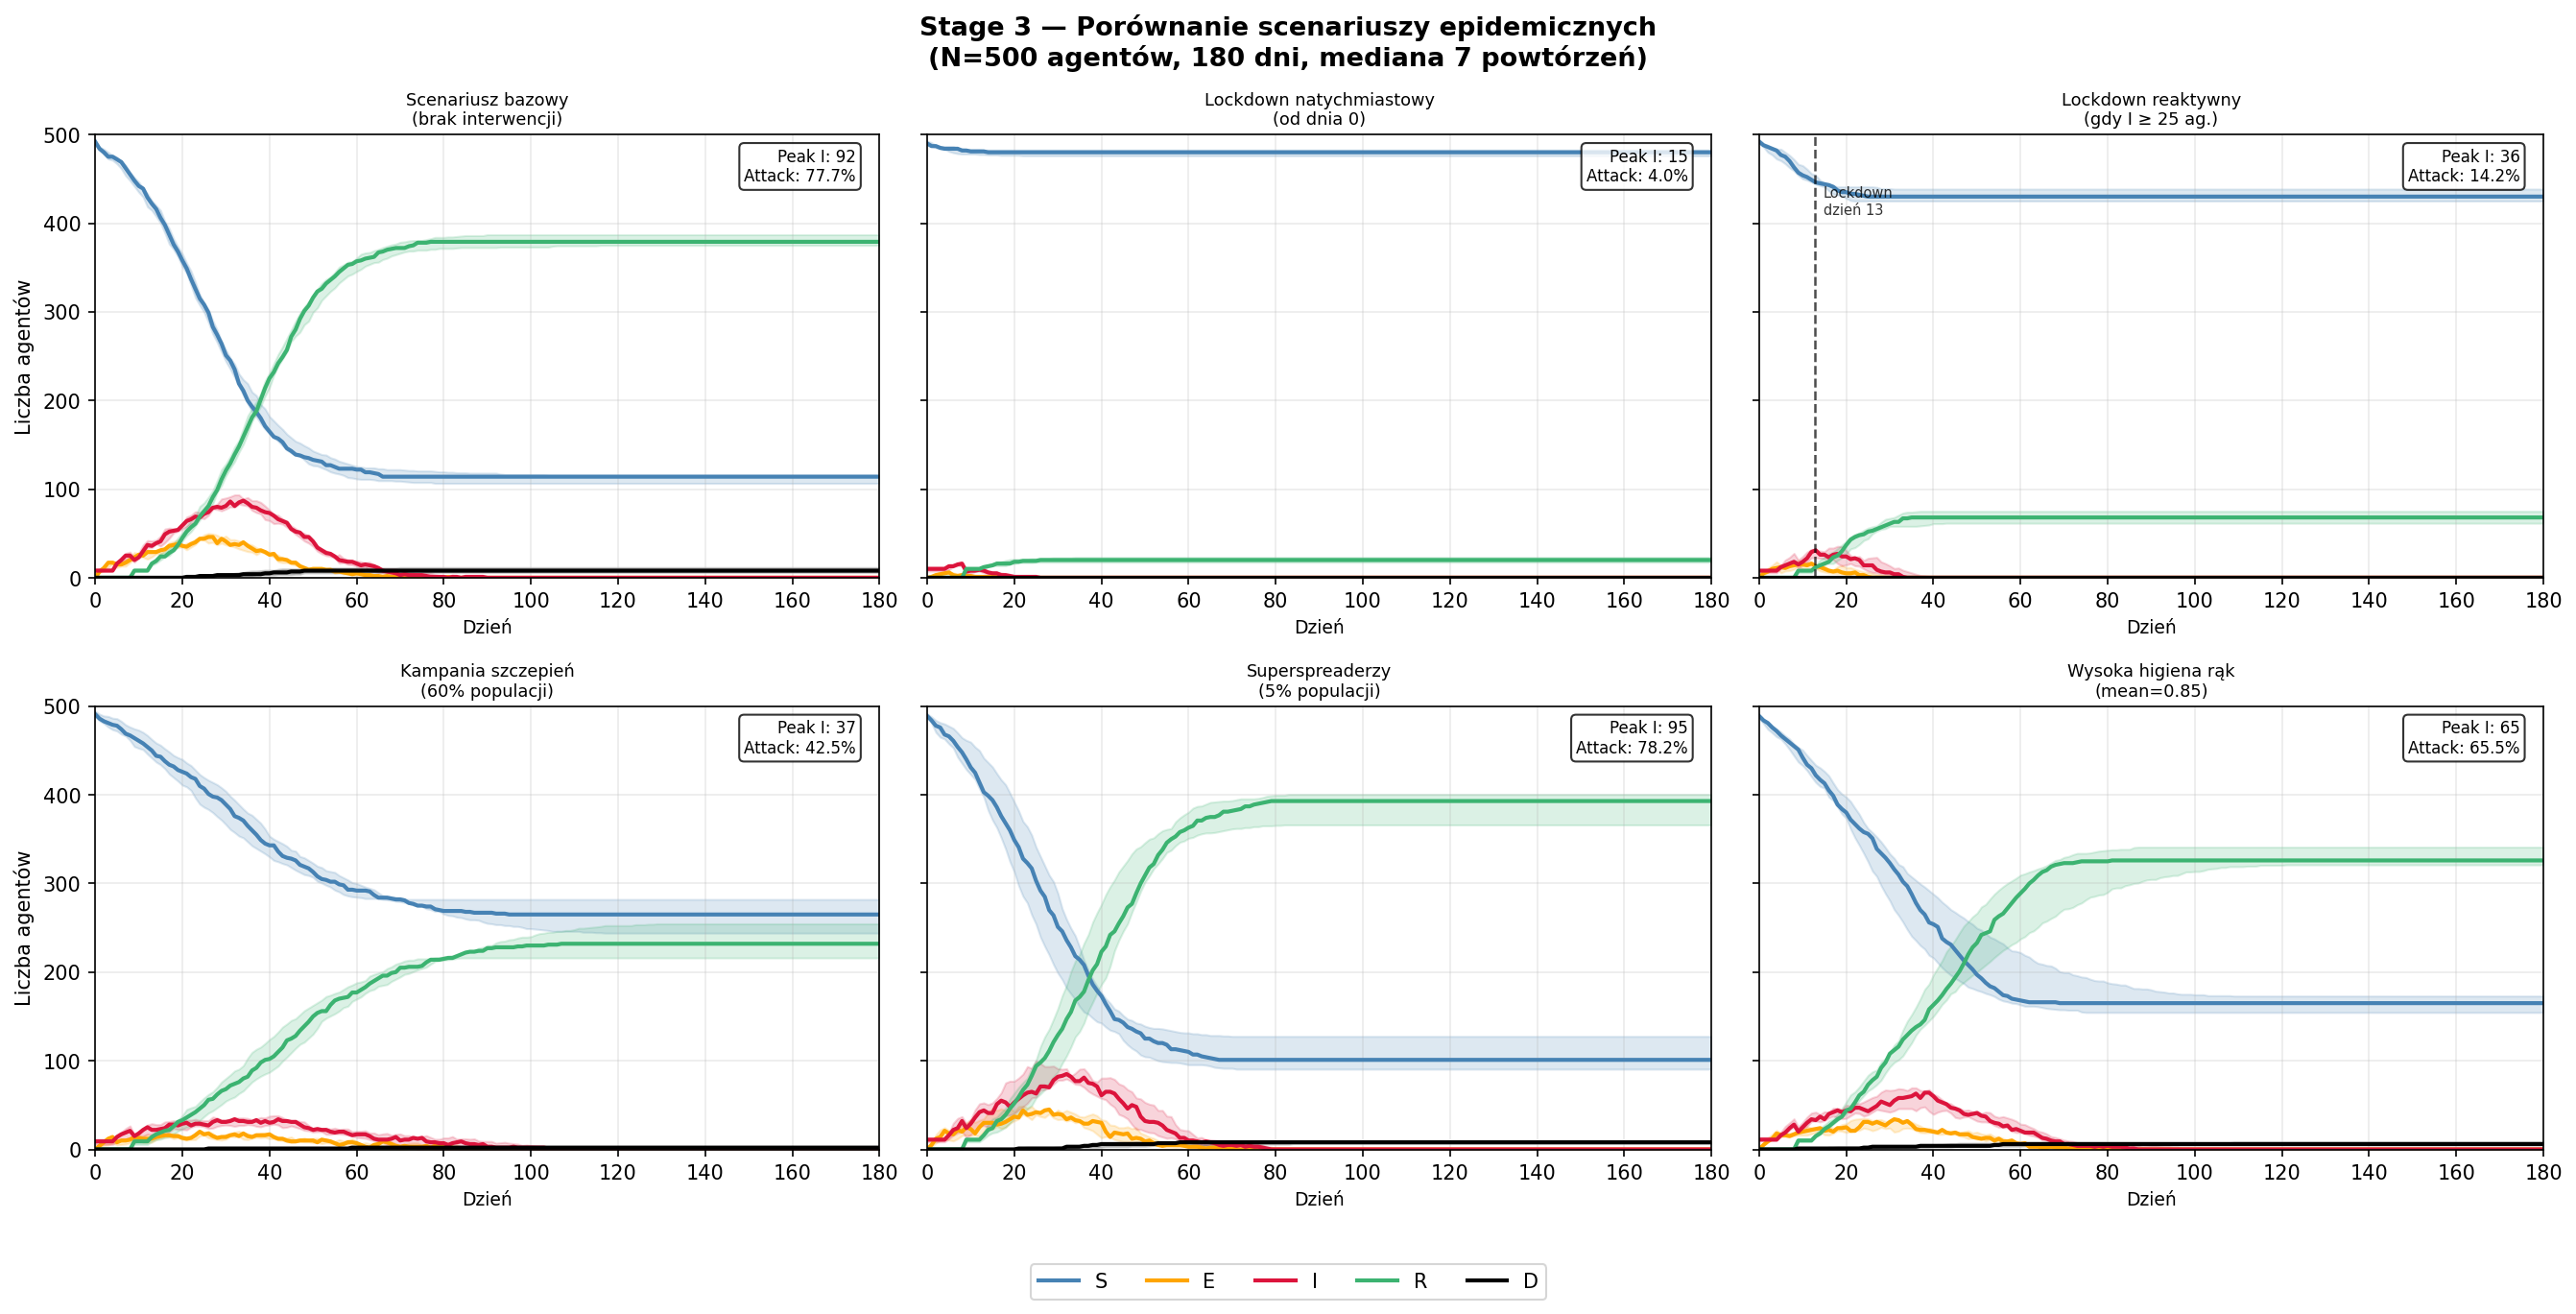
\includegraphics[width=\textwidth]{stage3_comparison.png}

    \vspace{0.1cm}
    {\small\textit{Krzywe I dla 5 scenariuszy -- mediana + IQR}}
  \end{columns}
\end{frame}

\begin{frame}{Wyniki: Szczepienia i Superspreaderzy}
  \begin{columns}[T]
    \column{0.50\textwidth}
    \textbf{Sc.~3 -- Szczepienia 60\%:}
    \begin{itemize}
      \item Attack rate: \textbf{49,1\%}\quad\textcolor{teal}{$\downarrow$35\%}
      \item Peak~I: \textbf{40} (dzień~42 -- opóźnienie!)
      \item Zgony: \textbf{3}\quad\textcolor{teal}{$\downarrow$55\%}
    \end{itemize}
    {\small Prog odporności stadnej: $1-1/R_0\approx60\%$ osiągnięty,
    lecz w~grupie niezaszczepionych tworzy się aktywny klaster.}

    \vspace{0.35cm}
    \textbf{Sc.~4 -- Superspreaderzy 5\%:}
    \begin{itemize}
      \item Attack rate: \textbf{78,7\%}\quad\textcolor{red}{$\uparrow$4 p.p.}
      \item Peak~I: \textbf{100} (1--2 dni wcześniej)
      \item Zasada \textbf{80/20} -- 25 agentów napędza ekspansję
    \end{itemize}

    \column{0.48\textwidth}
    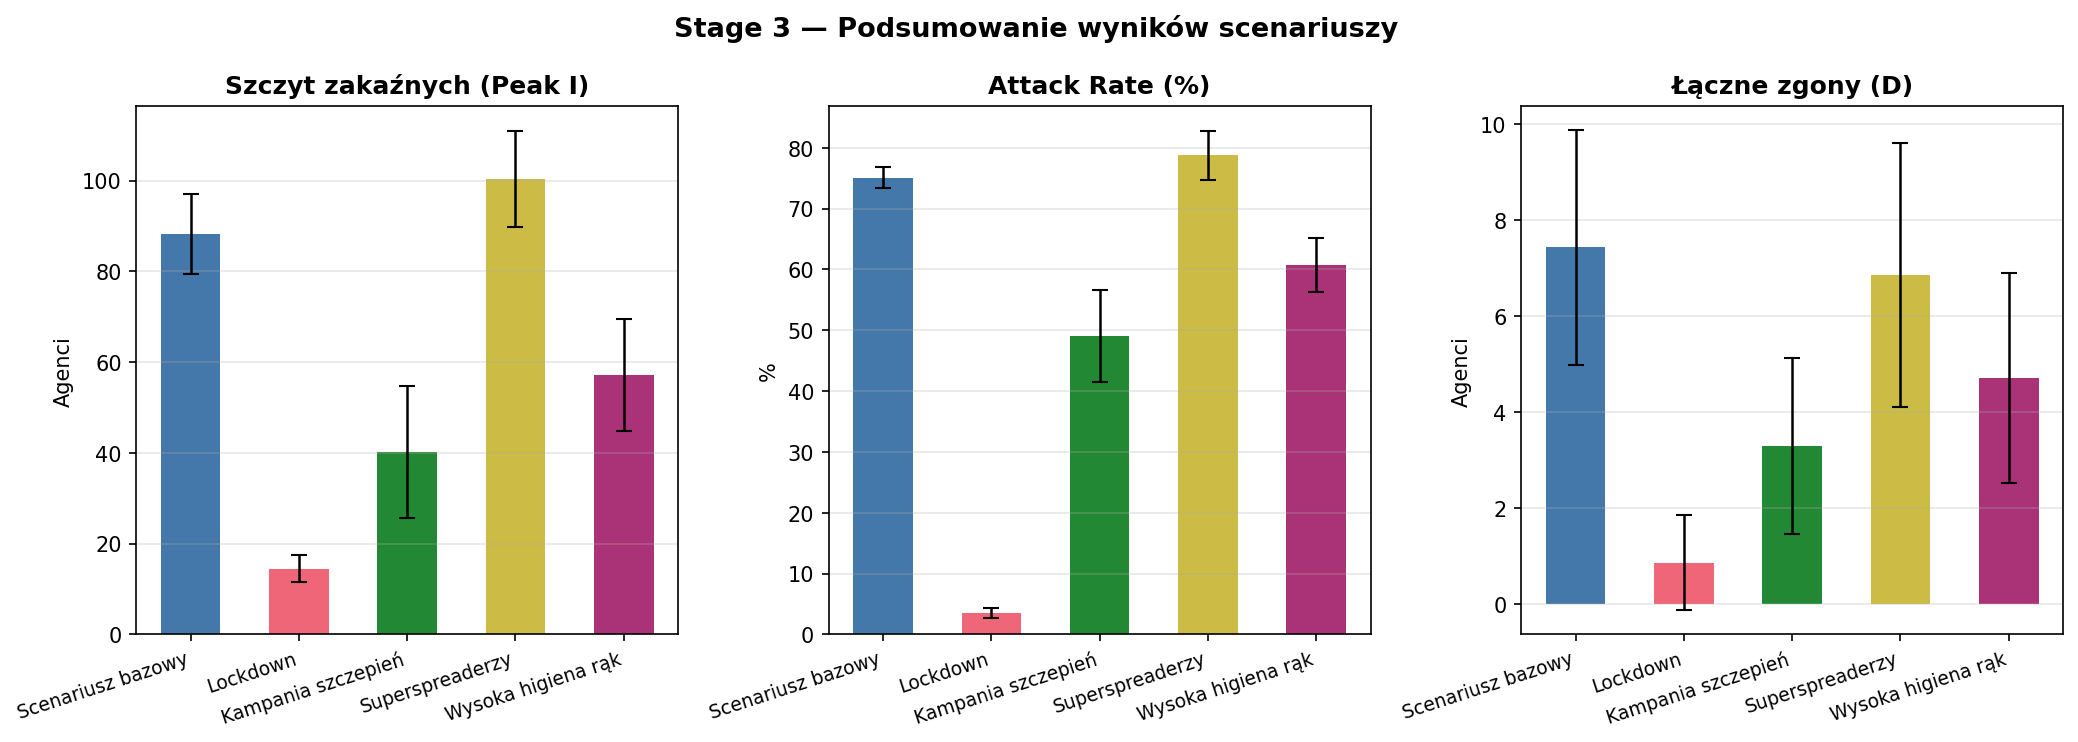
\includegraphics[width=\textwidth]{stage3_summary.png}

    \vspace{0.1cm}
    {\small\textit{Porównanie peak~I, attack rate i~zgonów}}
  \end{columns}
\end{frame}

\begin{frame}{Wyniki: Wpływ higieny rąk ($\Theta_H$)}
  \begin{columns}[T]
    \column{0.55\textwidth}
    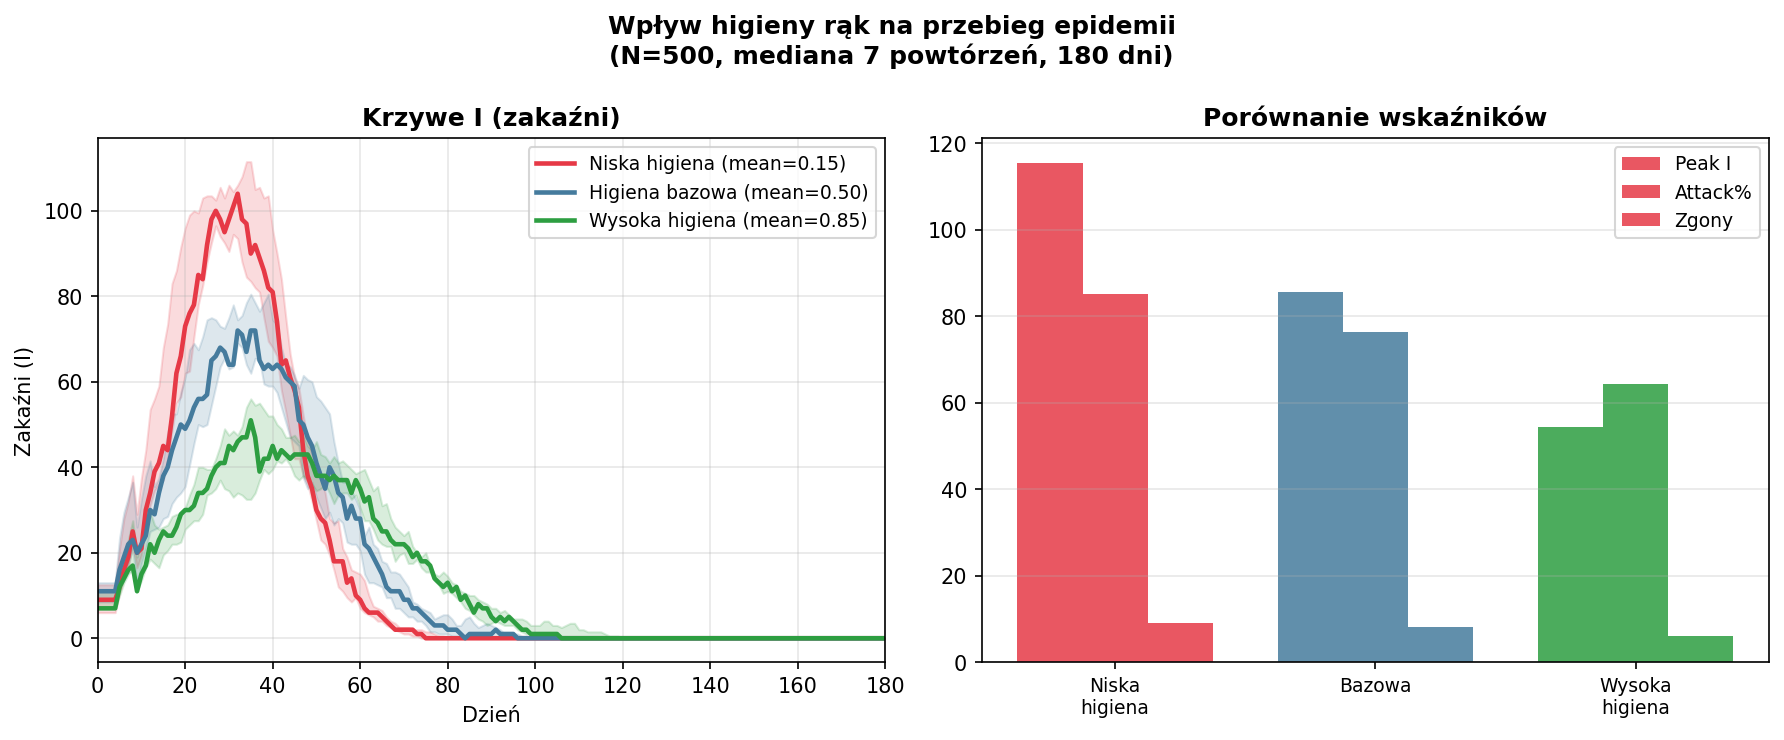
\includegraphics[width=\textwidth]{stage3_hygiene.png}

    \vspace{0.1cm}
    {\small\textit{Krzywe I i~wskaźniki dla trzech poziomów $\bar{\Theta}_H$}}

    \column{0.43\textwidth}
    \begin{tabular}{lcc}
      \toprule
      $\bar{\Theta}_H$ & AR & Peak~I (d.) \\
      \midrule
      0,15 (niska) & 85\% & 115\;(24) \\
      0,50 (baza)  & 76\% & 86\;(31) \\
      0,85 (wys.)  & 64\% & 54\;(42) \\
      \bottomrule
    \end{tabular}

    \vspace{0.4cm}
    \begin{block}{Wniosek}
      $\Delta\Theta_H = +0{,}35$:\\
      $-11$~p.p.\ attack rate\\
      $+18$~dni do szczytu
    \end{block}

    \vspace{0.2cm}
    Higiena \emph{spłaszcza} krzywą,\\
    ale nie eliminuje epidemii\\
    przy $R_0 > 1$.
  \end{columns}
\end{frame}

\begin{frame}{Wyniki zbiorcze}
  \begin{table}
    \centering
    \caption{Mediany wyników -- 5~scenariuszy, $N=500$, 7~powtórzeń, 180~kroków}
    \begin{tabularx}{\textwidth}{@{}lYYYY@{}}
      \toprule
      \textbf{Scenariusz} & \textbf{Attack rate} & \textbf{Peak~I} &
        \textbf{Dzień} & \textbf{Zgony} \\
      \midrule
      Bazowy            & 75,1\% & 88  & 31 & 7 \\
      \textbf{Lockdown} & \textbf{3,5\%} & \textbf{14} & 8 & \textbf{1} \\
      Szczepienia 60\%  & 49,1\% & 40  & 42 & 3 \\
      Superspreaderzy 5\% & 78,7\% & 100 & 31 & 7 \\
      Wysoka higiena    & 60,8\% & 57  & 42 & 5 \\
      \bottomrule
    \end{tabularx}
  \end{table}

  \vspace{0.3cm}
  \begin{columns}
    \column{0.5\textwidth}
    \textcolor{teal}{\textbf{Najskuteczniejsze:}} Lockdown ($-96\%$ AR)\\
    \textcolor{teal}{\textbf{Dobry kompromis:}} Szczepienia ($-35\%$ AR, $-55\%$ zgonów)

    \column{0.5\textwidth}
    \textcolor{orange}{\textbf{Częściowe:}} Wysoka higiena ($-14\%$ AR, $+11$~dni)\\
    \textcolor{red}{\textbf{Ryzyko:}} Superspreaderzy ($+4\%$ AR, wcześniejszy szczyt)
  \end{columns}
\end{frame}

% ============================================================
\section{Wnioski}

\begin{frame}{Wnioski końcowe}
  \begin{enumerate}
    \item \textbf{Lockdown jest najskuteczniejszą interwencją:}\\
          attack rate $75\% \to 3{,}5\%$ przez przecięcie wszystkich pozadomowych ścieżek.

    \vspace{0.25cm}
    \item \textbf{Szczepienia chronią głównie przed zgonem:}\\
          60\% pokrycia $\to$ $-35\%$ AR, $-55\%$ zgonów. Klaster w~grupie
          niezaszczepionych omija odporność stadną.

    \vspace{0.25cm}
    \item \textbf{Superspreaderzy przyspieszają epidemię:}\\
          5\% populacji (CR=3, $\Theta_H=0{,}1$) skraca czas do szczytu
          o~1--2~dni -- efekt zasady 80/20.

    \vspace{0.25cm}
    \item \textbf{Higiena spłaszcza krzywą, ale nie eliminuje epidemii:}\\
          $\Delta\Theta_H=+0{,}35$ $\Rightarrow$ $-21$~p.p.\ AR, $+18$~dni szczytu.
          Niewystarczające samodzielnie przy $R_0>1$.
  \end{enumerate}

  \vspace{0.25cm}
  \begin{block}{Główna przewaga ABM nad klasycznymi ODE}
    Możliwość badania \textbf{heterogenicznych} efektów interwencji
    -- rozkłady \texttt{contact\_rate} i~\texttt{hygiene\_score}
    wpływają na~makroskopową dynamikę epidemii w~sposób niedostępny
    w~modelach kompartmentowych.
  \end{block}
\end{frame}

\begin{frame}[plain]
  \vfill
  \begin{center}
    {\Huge Dziękuję za uwagę!}

    \vspace{1.2cm}

    {\large Dawid Mularczyk}\\[4pt]
    {\small Wydział Informatyki, Akademia Górniczo-Hutnicza}\\[4pt]
    {\small \texttt{muldaw@student.agh.edu.pl}}

    \vspace{1cm}
    {\normalsize Pytania?}
  \end{center}
  \vfill
\end{frame}

\end{document}
